\documentclass{article}
\usepackage[utf8]{inputenc}
\usepackage{amsmath}
\usepackage{amsfonts}
\usepackage{graphicx}

\title{Written Assignment Unit 4\\
Math 1201- College Algebra.
}
\author{Instructor - Casmir Onyeneke}
\date{September 2021}


\begin{document}

\maketitle

\section*{Question 1}
\title\textbf{Composite Functions}\\
Question Statement: What can be said about the domain of the function \textit f o g where ${\textit{f(y)} = \frac{4}{y-2}}$ and ${\textit{g(x)} = \frac{5}{3x-1}}$ ? Express in terms of a union of real numbers.\\
\textbf{Solution}
$${\textit{f(y)} = \frac{4}{y-2}}$$
$${\textit{g(x)} = \frac{5}{3x-1}}$$
\\The composite function \textit{f o g} can be expressed as

$${\textit{f o g} = \textit{f(g(x))}}$$
$${\textit{f o g} = \textit f\left(\frac{5}{3x-1}\right)}$$
$${\textit{f o g} = \frac{4}{\frac{5}{3x-1}-2}}$$
$${\textit{f o g} = \frac{4(3x-1)}{5 - (6x - 2)}}$$
$${\textit{f o g} = \frac{12x-4}{5 + 2 - 6x}}$$
$${\textit{f o g} = \frac{12x-4}{7 - 6x}}$$

The Domain of this composite function is:
$${7 - 6x \neq 0}$$
$${6x \neq 7}$$
$${x \neq \frac{7}{6}}$$
So therefore the domain expressed in interval notation is\\
$${(-\infty, \frac{7}{6})\cup(\frac{7}{6}, \infty)}$$ 
\\Below is the graph of \textit{f, g and f o g }\\
\\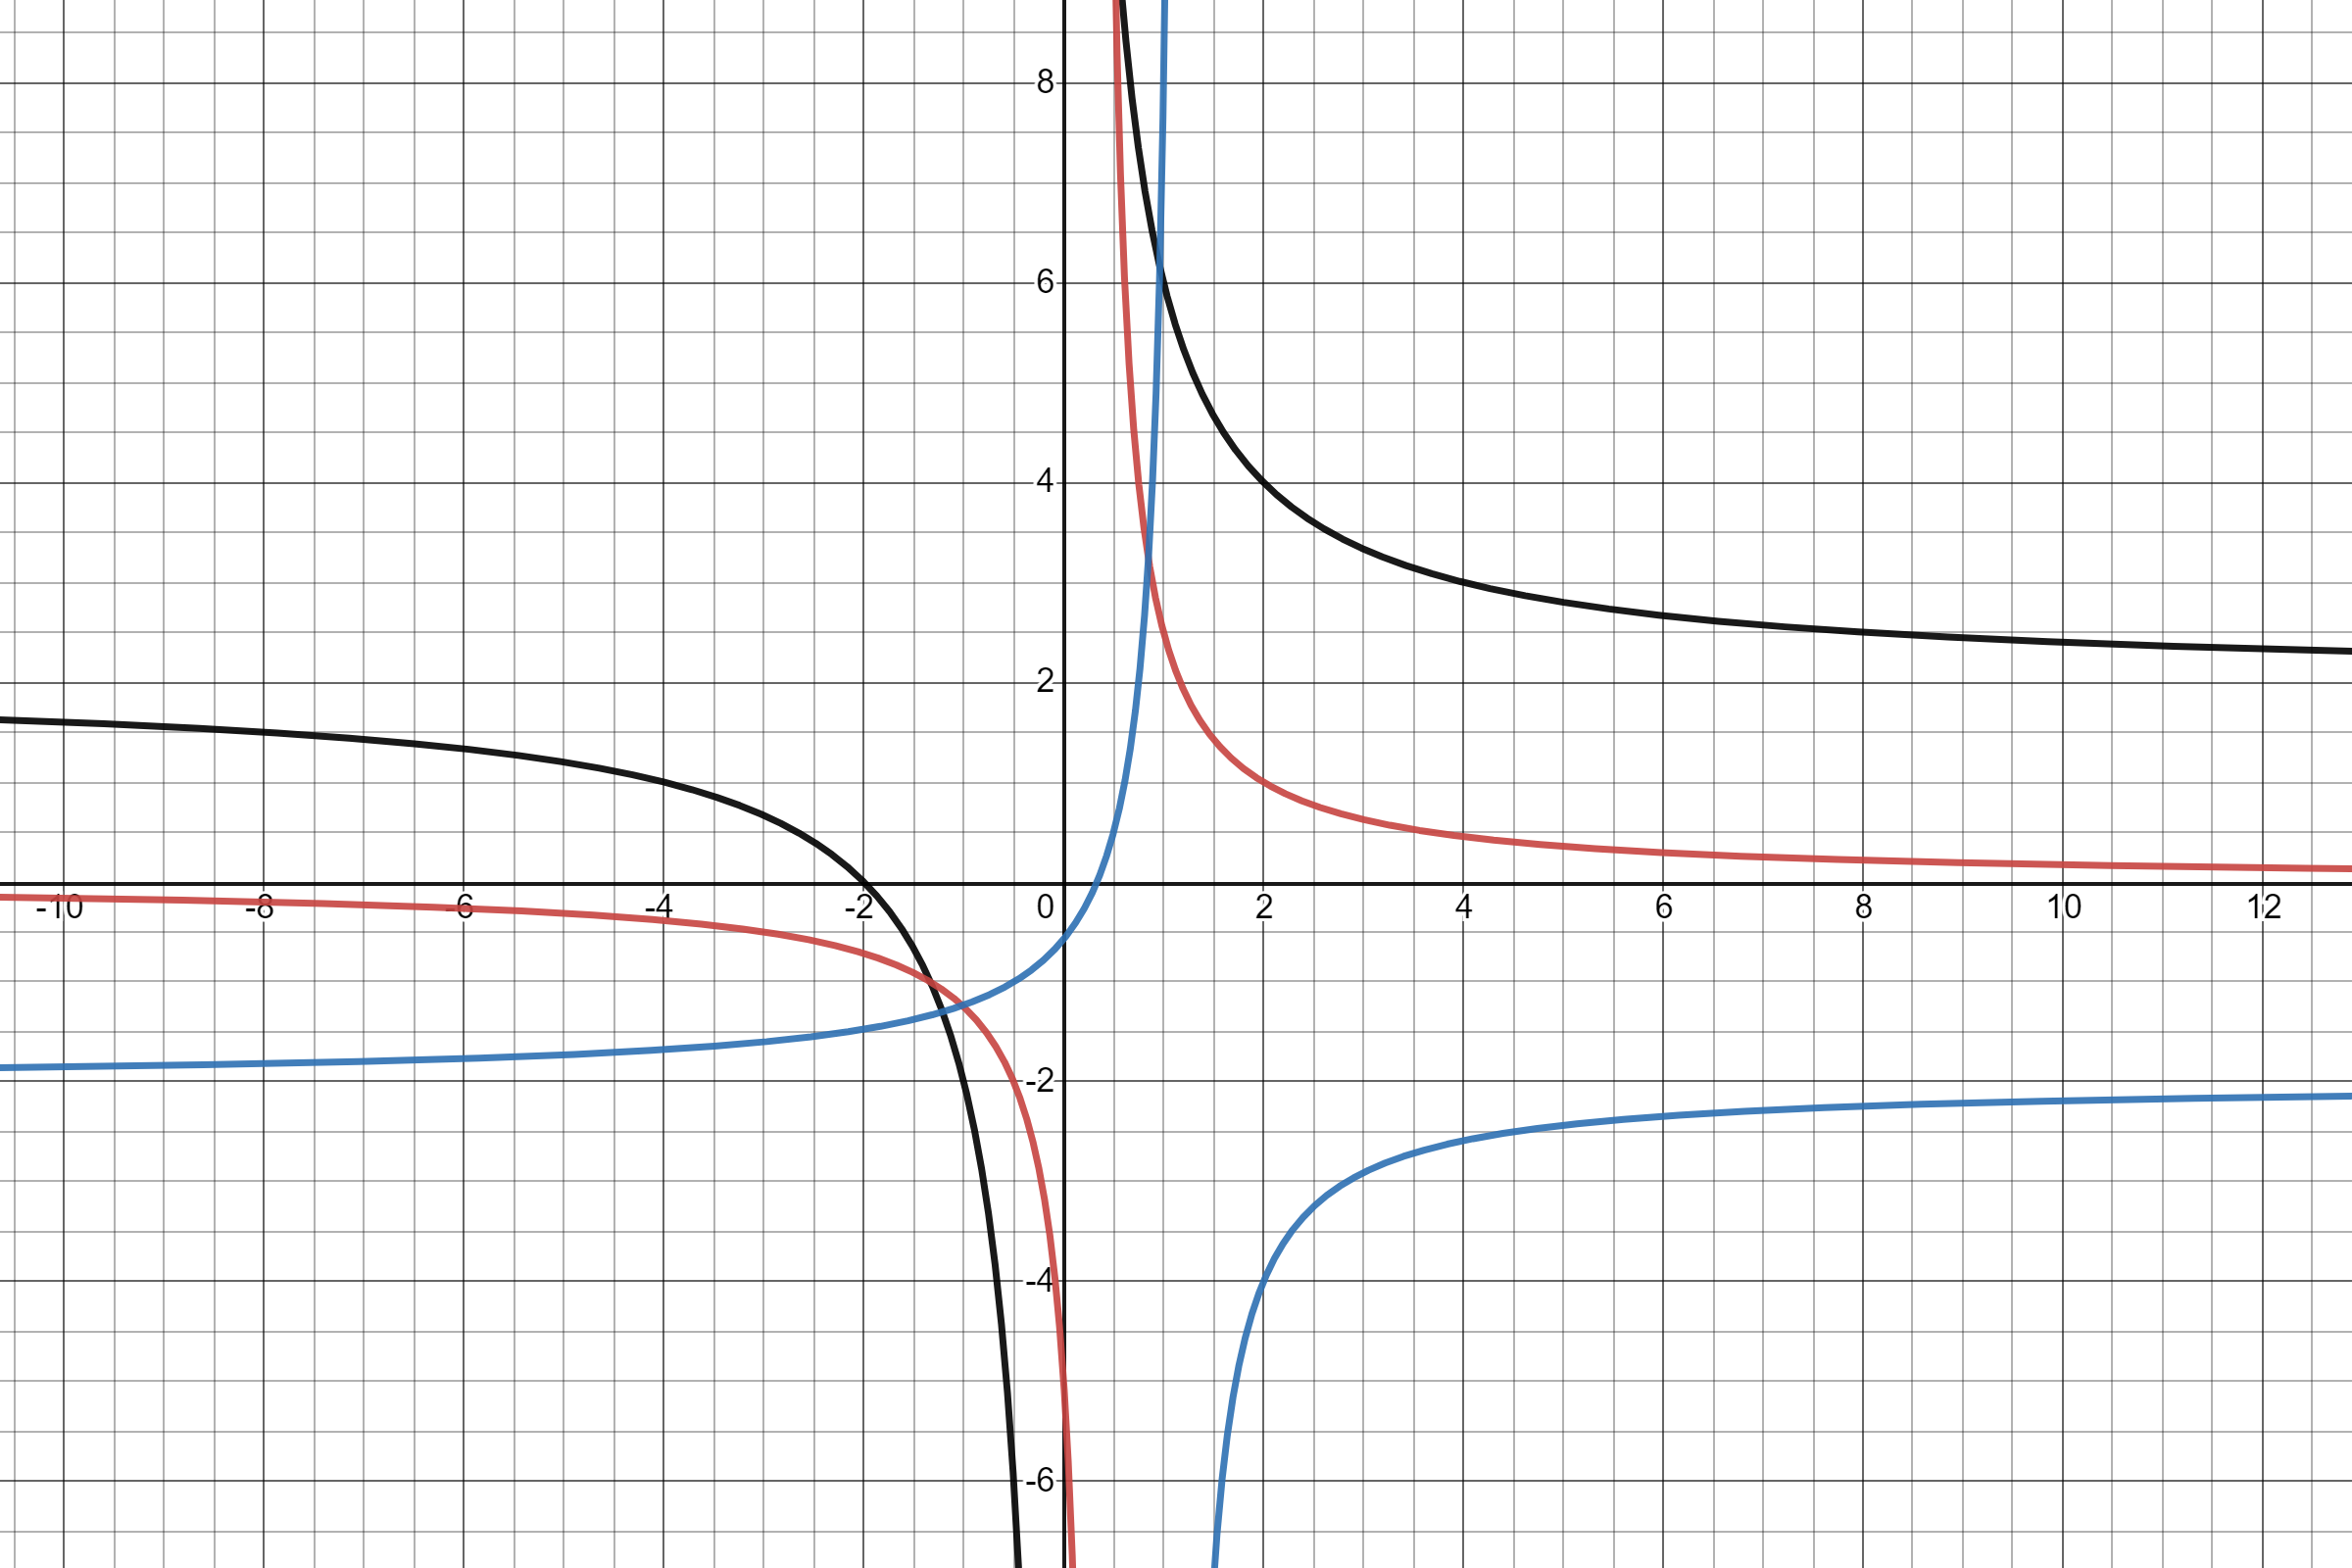
\includegraphics[scale = 0.15]{wAQ1}
\\$${\textit{f(y)} = \frac{4}{y-2}}$$
$${\textit{g(x)} = \frac{5}{3x-1}}$$
$${\textit{f o g} = \frac{12x-4}{7 - 6x}}$$
\section*{Question 2}
\title\textbf{Inverse Functions}
\\Question Statement: Find the inverse of the function ${\textit{f(x)}=4+\sqrt{x-2}}$
\\state the domains and ranges of both the function and the inverse function in terms of intervals of real numbers.
\\\textbf{Solution}
$${\textit{f(x)}=4+\sqrt{x-2}}$$
We can say that ${\textit{f(x)} = y}$
$${y = 4+\sqrt{x-2}}$$
Making ${x}$ the subject of the equation 
$${y = 4+\sqrt{x-2}}$$
subtract 4 from both the LHS and RHS
$${y - 4 = \sqrt{x-2}}$$
$${\sqrt{x-2} = y - 4 }$$
Square both the LHS and RHS
$${(\sqrt{x-2})^2 = (y - 4)^2 }$$
$${x - 2 = (y - 4)^2 }$$
Add 2 to both the LHS and RHS
$${x = (y - 4)^2 + 2}$$
\\Therefore the inverse function of ${\textit{f(x)}=4+\sqrt{x-2}}$  is  
${\textit f^{-1}(x) = (x - 4)^2 + 2 }$

\section*{Question 3}
\end{document}